% Options for packages loaded elsewhere
\PassOptionsToPackage{unicode}{hyperref}
\PassOptionsToPackage{hyphens}{url}
\PassOptionsToPackage{dvipsnames,svgnames,x11names}{xcolor}
\PassOptionsToPackage{space}{xeCJK}
\documentclass[
  10pt,
]{article}
\usepackage{xcolor}
\usepackage[margin=0.70in]{geometry}
\usepackage{amsmath,amssymb}
\setcounter{secnumdepth}{-\maxdimen} % remove section numbering
\usepackage{iftex}
\ifPDFTeX
  \usepackage[T1]{fontenc}
  \usepackage[utf8]{inputenc}
  \usepackage{textcomp} % provide euro and other symbols
\else % if luatex or xetex
  \usepackage{unicode-math} % this also loads fontspec
  \defaultfontfeatures{Scale=MatchLowercase}
  \defaultfontfeatures[\rmfamily]{Ligatures=TeX,Scale=1}
\fi
\usepackage{lmodern}
\ifPDFTeX\else
  % xetex/luatex font selection
  \setmainfont[]{Cambria}
  \setmonofont[]{Consolas}
  \ifXeTeX
    \usepackage{xeCJK}
    \setCJKmainfont[]{Microsoft YaHei}
  \fi
  \ifLuaTeX
    \usepackage[]{luatexja-fontspec}
    \setmainjfont[]{Microsoft YaHei}
  \fi
\fi
% Use upquote if available, for straight quotes in verbatim environments
\IfFileExists{upquote.sty}{\usepackage{upquote}}{}
\IfFileExists{microtype.sty}{% use microtype if available
  \usepackage[]{microtype}
  \UseMicrotypeSet[protrusion]{basicmath} % disable protrusion for tt fonts
}{}
\makeatletter
\@ifundefined{KOMAClassName}{% if non-KOMA class
  \IfFileExists{parskip.sty}{%
    \usepackage{parskip}
  }{% else
    \setlength{\parindent}{0pt}
    \setlength{\parskip}{6pt plus 2pt minus 1pt}}
}{% if KOMA class
  \KOMAoptions{parskip=half}}
\makeatother
\usepackage{longtable,booktabs,array}
\newcounter{none} % for unnumbered tables
\usepackage{calc} % for calculating minipage widths
% Correct order of tables after \paragraph or \subparagraph
\usepackage{etoolbox}
\makeatletter
\patchcmd\longtable{\par}{\if@noskipsec\mbox{}\fi\par}{}{}
\makeatother
% Allow footnotes in longtable head/foot
\IfFileExists{footnotehyper.sty}{\usepackage{footnotehyper}}{\usepackage{footnote}}
\makesavenoteenv{longtable}
\usepackage{graphicx}
\makeatletter
\newsavebox\pandoc@box
\newcommand*\pandocbounded[1]{% scales image to fit in text height/width
  \sbox\pandoc@box{#1}%
  \Gscale@div\@tempa{\textheight}{\dimexpr\ht\pandoc@box+\dp\pandoc@box\relax}%
  \Gscale@div\@tempb{\linewidth}{\wd\pandoc@box}%
  \ifdim\@tempb\p@<\@tempa\p@\let\@tempa\@tempb\fi% select the smaller of both
  \ifdim\@tempa\p@<\p@\scalebox{\@tempa}{\usebox\pandoc@box}%
  \else\usebox{\pandoc@box}%
  \fi%
}
% Set default figure placement to htbp
\def\fps@figure{htbp}
\makeatother
\setlength{\emergencystretch}{3em} % prevent overfull lines
\providecommand{\tightlist}{%
  \setlength{\itemsep}{0pt}\setlength{\parskip}{0pt}}
\usepackage{bookmark}
\IfFileExists{xurl.sty}{\usepackage{xurl}}{} % add URL line breaks if available
\urlstyle{same}
\hypersetup{
  colorlinks=true,
  linkcolor={Maroon},
  filecolor={Maroon},
  citecolor={Blue},
  urlcolor={Blue},
  pdfcreator={LaTeX via pandoc}}

\author{}
\date{}

\setlength{\textfloatsep}{10pt plus 2pt minus 2pt}
\begin{document}

\section{Eye Sentinel \textbar{} Missed referrals and paired
photographs}\label{eye-sentinel-missed-referrals-and-paired-photographs}

November 18, 2026 · \href{review-failures.zh.md}{中文} ·
\href{review-failures.en.pdf}{PDF}

\textbf{Using a second model to reorder negative calls increased the
missed referrals sent to review from 16 to 24.} Each rule reviewed 78 of
773 development photographs from AIROGS, a public glaucoma screening
dataset. EfficientNet-B0 made the initial calls. ResNet-50 helped
prioritize negative calls for review. The reference label indicates
whether a photo warrants referral. A miss is a negative call on a
referable photo, and a false positive is a referral call on a
nonreferable photo.

Uncertainty ranking prioritizes scores closest to the referral
threshold. The quality gray zone also gives priority to photos with
lower quality scores. Quality scores range from 0 to 1, with higher
values indicating better estimated quality. Two-model ranking keeps the
quality gray zone's positive review list and the number of negative
calls it reviews.

{\def\LTcaptype{none} % do not increment counter
\begin{longtable}[]{@{}
  >{\raggedright\arraybackslash}p{(\linewidth - 8\tabcolsep) * \real{0.1667}}
  >{\raggedright\arraybackslash}p{(\linewidth - 8\tabcolsep) * \real{0.1667}}
  >{\raggedleft\arraybackslash}p{(\linewidth - 8\tabcolsep) * \real{0.2222}}
  >{\raggedleft\arraybackslash}p{(\linewidth - 8\tabcolsep) * \real{0.2222}}
  >{\raggedleft\arraybackslash}p{(\linewidth - 8\tabcolsep) * \real{0.2222}}@{}}
\toprule\noalign{}
\begin{minipage}[b]{\linewidth}\raggedright
Photo mix
\end{minipage} & \begin{minipage}[b]{\linewidth}\raggedright
Review rule
\end{minipage} & \begin{minipage}[b]{\linewidth}\raggedleft
All errors reviewed
\end{minipage} & \begin{minipage}[b]{\linewidth}\raggedleft
Misses reviewed
\end{minipage} & \begin{minipage}[b]{\linewidth}\raggedleft
Misses left per 1,000
\end{minipage} \\
\midrule\noalign{}
\endhead
\bottomrule\noalign{}
\endlastfoot
Original mix & Uncertainty & 32.8\% & 30.0\% & 45.3 \\
& Quality gray zone & 32.8\% & 32.0\% & 44.0 \\
& Two-model ranking & 44.8\% & 48.0\% & 33.6 \\
3.2\% positive & Uncertainty & 57.5\% & 44.0\% & 2.4 \\
& Quality gray zone & 63.2\% & 48.0\% & 2.2 \\
& Two-model ranking & 65.2\% & 70.0\% & 1.3 \\
\end{longtable}
}

The development set contained 380 referable photos. The 3.2\% scenario
changes their weight to match the public AIROGS training share and
reviews 100 photos per 1,000. Coverage divides reviewed errors by the
initial errors of that type. Misses left per 1,000 uses all photos.
Compared with the quality gray zone, two-model ranking sent 8 extra
misses to review, with a 95\% interval of {[}1, 12{]}. At 3.2\%
positives, the gain was 0.93 per 1,000 {[}0.09, 1.60{]}. To estimate the
intervals, we resampled same-patient or related photos together and
compared both rules on each draw.
\href{https://arxiv.org/html/2302.01738}{Original AIROGS study}

\begin{figure}
\centering
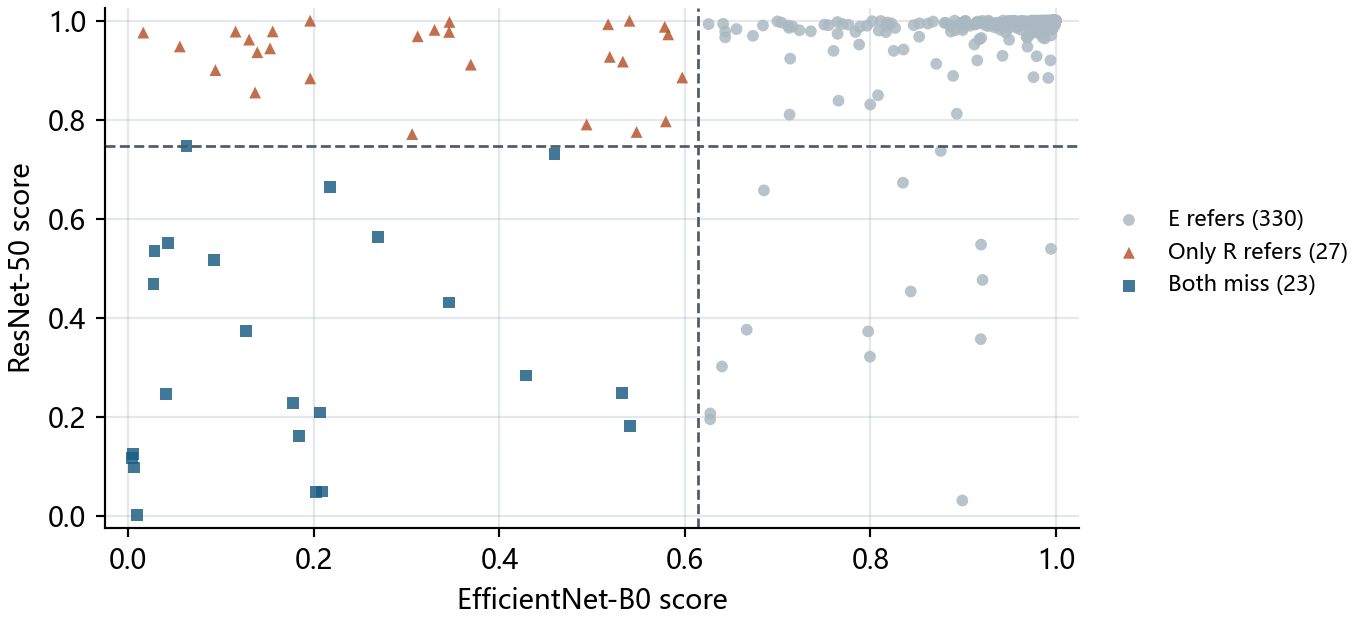
\includegraphics[width=0.88\linewidth,height=\textheight,keepaspectratio,alt={Each point represents a referable photo. E is EfficientNet-B0 and R is ResNet-50. Each model calls a photo positive above its own dashed threshold.}]{review-model-disagreement.en.png}
\caption{Each point represents a referable photo. E is EfficientNet-B0
and R is ResNet-50. Each model calls a photo positive above its own
dashed threshold.}
\end{figure}

EfficientNet-B0 initially missed 50 photographs. ResNet-50 flagged 27,
including 15 of the 34 misses outside the quality gray zone. Both models
called the other 19 outside-review misses negative. Both saved models
came from update 2,400. We fit the combined score on 767 validation
photos and evaluated it on a separate set of 773 development photos.
\href{backbone-comparison.en.md}{Matched training record}

\newpage

\subsection{How image quality moves the
score}\label{how-image-quality-moves-the-score}

We applied two levels of simulated blur to the same 773 AIROGS photos
and kept the original disease classification threshold. Misses changed
from \textbf{50/380} on original photos to \textbf{109/380} and
\textbf{230/380}. Under strong blur, scores fell on 348/380 and rose on
32/380 reference-positive photos. 185 crossed from a positive call to a
miss and 5 changed in the reverse direction. Scores rose on 340/393
reference-negative photos. The scores moved in opposite directions
across the two reference classes, making the initially high-scoring
positives and low-scoring negatives harder to tell apart.

\begin{figure}
\centering
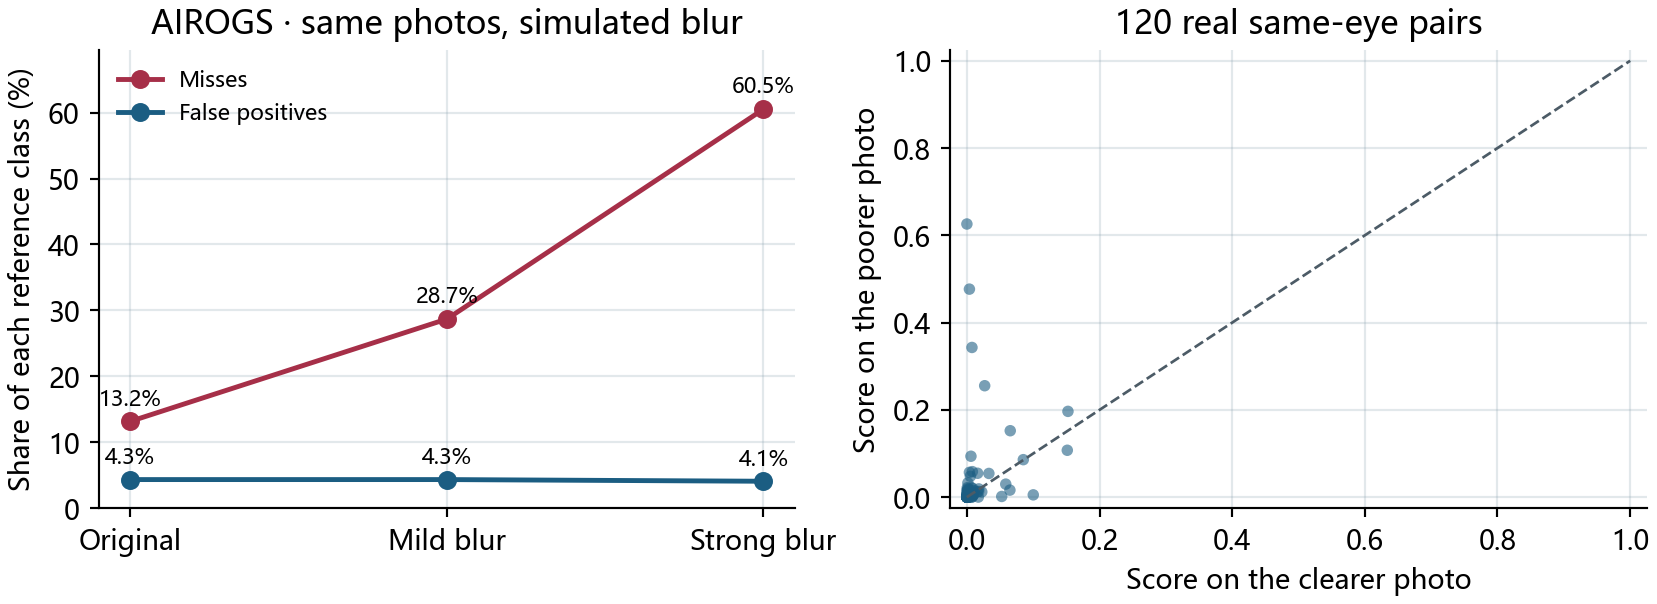
\includegraphics[width=0.98\linewidth,height=\textheight,keepaspectratio,alt={The left panel shows simulated blur on labeled AIROGS photos. The right panel shows clearer and poorer same-eye photos from Real Fundus. The dashed line indicates equal scores.}]{review-paired-focus.en.png}
\caption{The left panel shows simulated blur on labeled AIROGS photos.
The right panel shows clearer and poorer same-eye photos from Real
Fundus. The dashed line indicates equal scores.}
\end{figure}

Among \textbf{120 real same-eye pairs} in Real Fundus, the poorer photo
scored \textbf{lower in 45 pairs and higher in 75}. Only 1 pair crossed
the threshold, from a negative call on the clearer photo to a positive
call on the poorer photo. Real pairs can vary in focus, illumination and
framing. The release supplies image-quality pairs without a glaucoma
reference for this analysis. The results measure sensitivity to the
choice of photo. \href{https://arxiv.org/abs/2201.00466}{Real Fundus
study}

One referable photo had distinct vessel outlines and a quality score of
0.89. Its referral scores of 0.35 and 0.43 were below both models'
thresholds, and the photo remained outside review. A reader could assess
the optic disc, where the optic nerve leaves the eye, and its central
depression, the optic cup, without seeing the model calls.

\subsection{Next validation}\label{next-validation}

Keep the current quality gray zone as the comparison. Collect first and
repeat photos with an independent clinical reference and record whether
the disc and cup can be judged. In consecutive patients at the intended
site, measure misses and net corrections at ten reviews per hundred
patients. Net corrections are model errors the reader fixes minus new
reader errors. This analysis measures which photos reach review using
one training run per model. Reader corrections and the benefit of
retakes remain to be measured. The independent test sets remain sealed.

\href{review-failures-results.json}{Results and input hashes} ·
\href{../../../tools/analyze_review_failures_20261118.py}{Analysis} ·
\href{../../../tools/plot_review_failures_20261118.py}{Figures}

\end{document}
